\chapter{Eigenabstand, Kruskal-Geometrie und Beobachter am Horizont}

Die Schwarzschild-Metrik scheint am Horizont singulär zu werden. Die Krümmung tut das nicht. Um diese beiden Aussagen auseinanderzuhalten, entfernen wir zunächst den Gesamtskalierungsfaktor des Schwarzen Lochs und ersetzen dann die radiale Koordinate durch den Eigenabstand vom Horizont. In Horizontnähe ist die resultierende Geometrie gewöhnliche flache Raumzeit in beschleunigten Koordinaten. Ist diese Geometrie erst einmal gezeichnet, werden Fragen zu Alice, Bob und Charlie zu Fragen über Weltlinien und Lichtstrahlen statt zu verbalen Paradoxien.

\section{Den Schwarzschild-Radius herausfaktorisieren}

Wir beginnen mit gestrichenen Koordinaten, damit die skalierten Variablen später die vertrauten Namen tragen können:
\begin{equation}
d\tau^2
=
\left(1-\frac{2MG}{r'}\right)dt'^2
-
\frac{dr'^2}{1-\frac{2MG}{r'}}
-
r'^2d\Omega_2^2.
\label{eq:l7-schwarzschild-dimensional}
\end{equation}
Wir führen den Schwarzschild-Radius und dimensionslose Koordinaten ein:
\begin{equation}
r_{\mathrm S}=2MG,
\qquad
r=\frac{r'}{r_{\mathrm S}},
\qquad
t=\frac{t'}{r_{\mathrm S}}.
\label{eq:l7-rescaling}
\end{equation}
Wir verwenden \(c=1\), sodass Zeit und Länge dieselben Einheiten haben. Der Radius \(r_{\mathrm S}\) ist daher sowohl eine Länge als auch die zugehörige Lichtlaufzeit. Einsetzen ergibt
\begin{equation}
d\tau^2
=r_{\mathrm S}^2
\left[
\left(1-\frac1r\right)dt^2
-
\frac{dr^2}{1-\frac1r}
-
r^2d\Omega_2^2
\right].
\label{eq:l7-schwarzschild-rescaled}
\end{equation}
Alle nichtrotierenden, ungeladenen Schwarzschild-Schwarzen-Löcher haben folglich dieselbe dimensionslose Geometrie. Eine Änderung der Masse ändert den Maßstab, mit dem die Metrik multipliziert wird, nicht aber die Form des Ausdrucks in den Klammern. Das ist so, als zeichnete man Kugeln, nachdem man alle Abstände durch den jeweiligen Kugelradius geteilt hat: Dieselbe Zeichnung beschreibt den Mond und die Erde, obwohl ein Zentimeter in der einen Zeichnung einem anderen physikalischen Abstand entspricht als in der anderen.

\begin{classroomqa}
\audiencequestion{Welche Vorzeichen haben die radialen und die winkelabhängigen Terme der Metrik?}
\lecturerresponse{Bei der hier verwendeten Signatur \(+---\) tragen beide räumlichen Terme ein Minuszeichen. Der Raum fing den Vorzeichenfehler auf, als der Ausdruck angeschrieben wurde. Der Winkelfaktor kann je nach Konvention einen Sinus oder einen Kosinus enthalten, je nachdem, ob die Polarkoordinate von der Achse oder vom Äquator aus gemessen wird; die kompakte Schreibweise \(d\Omega_2^2\) umgeht diese Konventionsfrage.
\lecturetimestamp{00:07:48--00:08:12}}
\end{classroomqa}

\section{Die Krümmungsskala am Horizont}

Die Reskalierung beantwortet eine wichtige physikalische Frage, ohne dass eine lange Tensorrechnung nötig ist. Eine Metrikkomponente ist dimensionslos. Ein Christoffel-Symbol enthält eine Koordinatenableitung und hat daher die Dimension einer inversen Länge, während eine Komponente des Riemann-Tensors in einem physikalischen orthonormalen Bezugssystem die Dimension
\begin{equation}
[g_{\mu\nu}]=1,
\qquad
[\Gamma^\mu{}_{\nu\rho}]=L^{-1},
\qquad
[R_{\hat\alpha\hat\beta\hat\gamma\hat\delta}]
=L^{-2}.
\label{eq:l7-curvature-dimensions}
\end{equation}
hat. Am Horizont \(r=1\) ist \(r_{\mathrm S}\) die einzige verfügbare physikalische Länge. Die Gezeitenkrümmung muss daher die Skala
\begin{equation}
\left|R_{\hat\alpha\hat\beta\hat\gamma\hat\delta}\right|_{\mathrm{hor}}
\sim \frac{1}{r_{\mathrm S}^2}.
\label{eq:l7-horizon-curvature}
\end{equation}
haben. Allgemeiner ist sie \(r_{\mathrm S}^{-2}\) multipliziert mit einer dimensionslosen Funktion von \(r\). Diese Aussage betrifft das Riemannsche Gezeitenfeld, nicht den Ricci-Skalar, der im Schwarzschild-Vakuum verschwindet.

Die physikalische Schlussfolgerung liegt unmittelbar auf der Hand. Mit zunehmender Masse wächst \(r_{\mathrm S}\), und das Gezeitenfeld am Horizont wird schwächer. Ein kleines Schwarzes Loch kann einen ausgedehnten Körper beim Durchqueren auseinanderreißen; nahe dem Horizont eines supermassereichen Schwarzen Lochs können die Gezeitenkräfte mild sein. Nach innen nimmt die Krümmung dennoch zu und divergiert bei \(r=0\). Horizont und Singularität sind daher grundverschieden.

\section{Eigenabstand vom Horizont}

Für den Rest der lokalen Rechnung setzen wir \(r_{\mathrm S}=1\). Koordinatenwechsel sind in der Relativitätstheorie keine bloße Kosmetik: Eine ungünstige Koordinate kann eine reguläre Geometrie hinter singulären Koeffizienten verbergen. Die Schwarzschild-Koordinatendifferenz \(r-1\) ist nicht der gemessene radiale Abstand vom Horizont.

\begin{figure}[htbp]
\centering
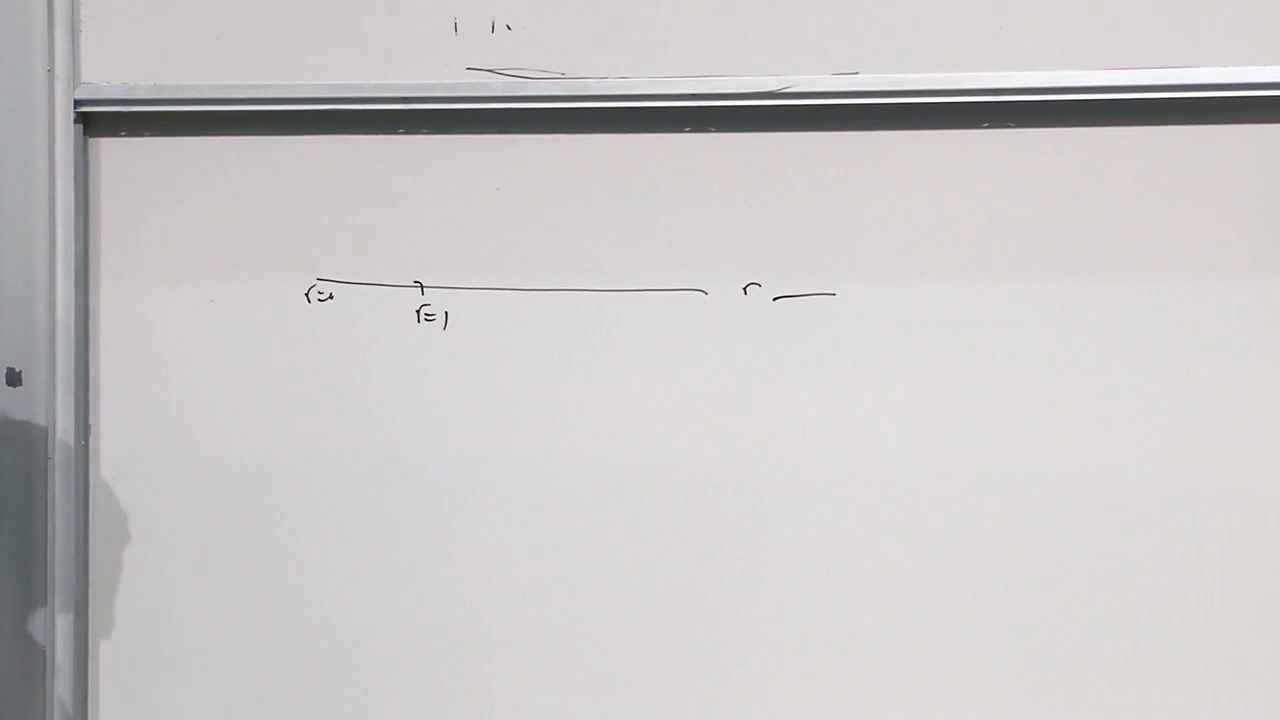
\includegraphics[width=0.78\textwidth]{lecture_07_figure_02.png}
\caption{Die am Tafelbild verwendete radiale Koordinatenlinie. Der Horizont liegt bei \(r=1\), während \(r=0\) die Krümmungssingularität ist.}
\lectureframe{00:16:11}
\end{figure}

Wir halten \(t\) und die Winkel fest. Dann lautet das positive räumliche Linienelement
\begin{equation}
ds^2=\frac{dr^2}{1-\frac1r},
\qquad
ds=\sqrt{\frac{r}{r-1}}\,dr.
\label{eq:l7-radial-proper-line}
\end{equation}
Den dimensionslosen Eigenabstand vom Horizont definieren wir durch
\begin{equation}
\rho(r)
=
\int_1^r\sqrt{\frac{r'}{r'-1}}\,dr'.
\label{eq:l7-rho-definition}
\end{equation}
Der physikalische Abstand ist \(r_{\mathrm S}\rho\), wenn wir den Gesamtmaßstab wieder einsetzen. Die geschlossene Form des Integrals brauchen wir nicht. Es genügt seine Ableitung:
\begin{equation}
\frac{d\rho}{dr}
=\sqrt{\frac{r}{r-1}},
\qquad
d\rho^2
=\frac{dr^2}{1-\frac1r}.
\label{eq:l7-rho-derivative}
\end{equation}
Damit wird der komplizierte radiale Term exakt zu \(-d\rho^2\). Genau deshalb führen wir \(\rho\) ein.

Nun skalieren wir die Zeitkoordinate ein weiteres Mal um:
\begin{equation}
\omega=\frac{t}{2}.
\label{eq:l7-omega}
\end{equation}
Da \(r\) eine Funktion von \(\rho\) ist, lässt sich die Metrik schreiben als
\begin{equation}
d\tau^2
=
F(\rho)\rho^2d\omega^2
-
d\rho^2
-
r(\rho)^2d\Omega_2^2.
\label{eq:l7-rho-metric}
\end{equation}

\begin{classroomqa}
\audiencequestion{Wird \(F(\rho)\) einfach so definiert, dass der Zeitkoeffizient die Form \(F(\rho)\rho^2\) hat?}
\lecturerresponse{Ja. An dieser Stelle hat die Faktorisierung keinen eigenständigen physikalischen Gehalt. Sie ist eine zweckmäßige Definition. Nützlich wird sie, wenn man die Grenzwerte von \(F\) nahe am und weit entfernt vom Horizont betrachtet.
\lecturetimestamp{00:26:39--00:26:59}}
\end{classroomqa}

Weit entfernt geht der Zeitkoeffizient der Schwarzschild-Metrik gegen eins. Wegen \(dt=2d\omega\) wird daraus
\begin{equation}
\lim_{\rho\to\infty}F(\rho)\rho^2=4.
\label{eq:l7-far-limit}
\end{equation}
Nahe am Horizont ergibt Gl.~\eqref{eq:l7-rho-definition}
\begin{equation}
\begin{aligned}
\rho&\simeq 2\sqrt{r-1},\\
r(\rho)&=1+\frac{\rho^2}{4}+O(\rho^4),\\
\lim_{\rho\to0}F(\rho)&=1.
\end{aligned}
\label{eq:l7-near-expansion}
\end{equation}

\begin{figure}[htbp]
\centering
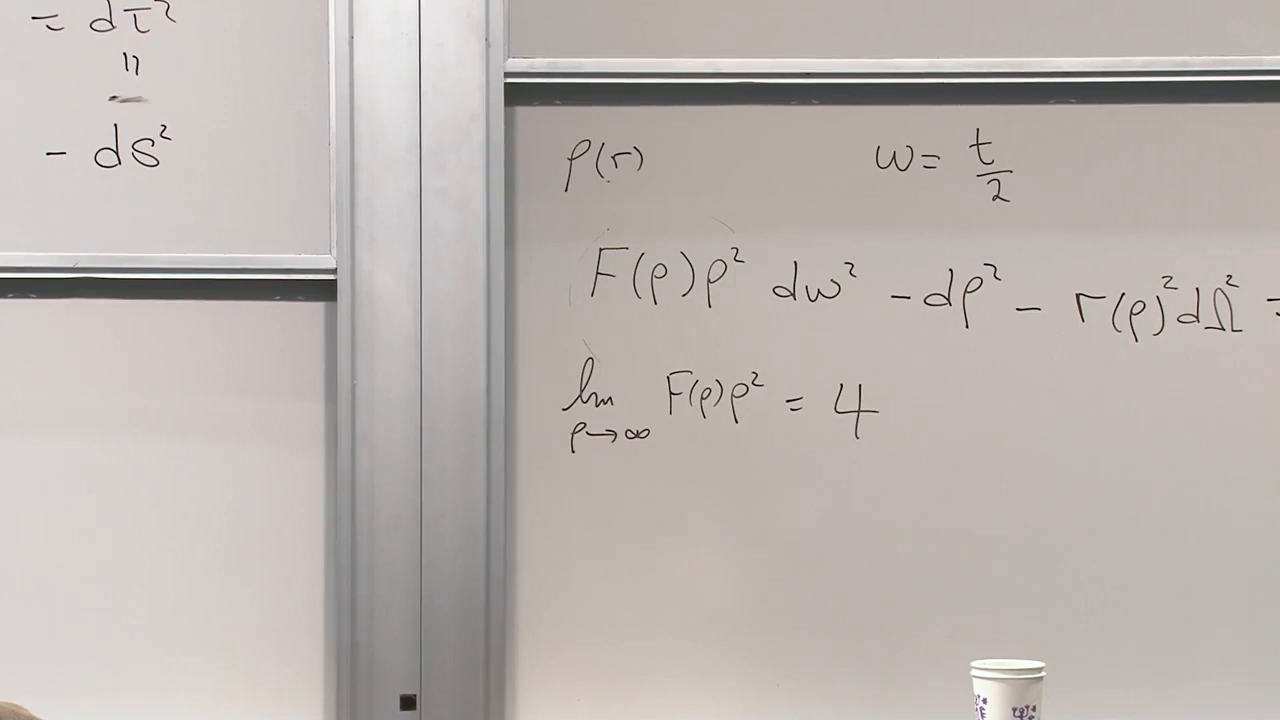
\includegraphics[width=0.90\textwidth]{lecture_07_figure_03.png}
\caption{Die Metrik in \((\rho,\omega)\), ihr asymptotischer Zeitkoeffizient sowie die Grenzwerte nahe am Horizont \(F\to1\) und \(r=1+\rho^2/4+\cdots\).}
\lectureframe{00:37:30}
\end{figure}

\section{Flache Raumzeit, verborgen am Horizont}

Nahe bei \(\rho=0\) geht der radial-zeitliche Anteil von Gl.~\eqref{eq:l7-rho-metric} über in
\begin{equation}
d\tau_{\mathrm{radial}}^2
\simeq
\rho^2d\omega^2-d\rho^2.
\label{eq:l7-rindler-metric}
\end{equation}
Das ist flache Minkowski-Raumzeit in hyperbolischen Polarkoordinaten. Wir definieren
\begin{equation}
X=\rho\cosh\omega,
\qquad
T=\rho\sinh\omega.
\label{eq:l7-rindler-transform}
\end{equation}
Dann gilt
\begin{equation}
dT^2-dX^2
=
\rho^2d\omega^2-d\rho^2.
\label{eq:l7-minkowski-check}
\end{equation}
Kurven mit konstantem \(\rho\) erfüllen
\begin{equation}
X^2-T^2=\rho^2
\label{eq:l7-constant-rho}
\end{equation}
und sind Hyperbeln. Kurven mit konstantem \(\omega\) sind Strahlen vom Ursprung. Für \(\omega\to\infty\) nähern sich diese Strahlen der lichtartigen Geraden \(T=X\) an. Der Schwarzschild-Horizont, der scheinbar auf unendliche Koordinatenzeit verschoben ist, ist daher im regulären Diagramm eine gewöhnliche lichtartige Gerade.

\begin{figure}[htbp]
\centering
\includegraphics[width=0.88\textwidth]{lecture_07_figure_06.png}
\caption{Die fertiggestellte Geometrie auf der Tafel: Hyperbeln mit konstantem \(\rho\), Strahlen mit konstantem \(\omega\), der lichtartige Horizont und der Bereich \(r<1\) darüber.}
\lectureframe{00:38:30}
\end{figure}

\begin{figure}[htbp]
\centering
\resizebox{0.96\linewidth}{!}{%
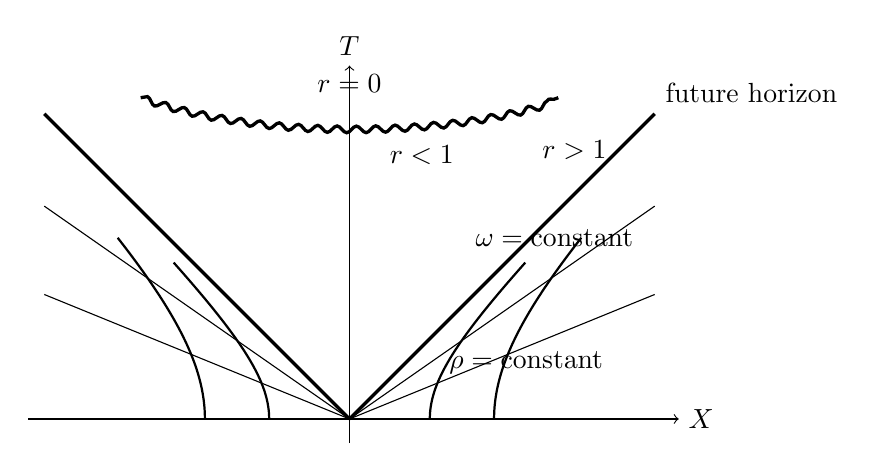
\begin{tikzpicture}[scale=1.02]
\draw[->] (-4.0,0) -- (4.1,0) node[right] {$X$};
\draw[->] (0,-0.3) -- (0,4.4) node[above] {$T$};
\draw[very thick] (0,0) -- (3.8,3.8)
  node[above right] {future horizon};
\draw[very thick] (0,0) -- (-3.8,3.8);
\draw[thick]
  plot[domain=0:1.42,samples=50]
  ({1.0*cosh(\x)},{1.0*sinh(\x)});
\draw[thick]
  plot[domain=0:1.05,samples=50]
  ({1.8*cosh(\x)},{1.8*sinh(\x)});
\draw[thick]
  plot[domain=0:1.42,samples=50]
  ({-1.0*cosh(\x)},{1.0*sinh(\x)});
\draw[thick]
  plot[domain=0:1.05,samples=50]
  ({-1.8*cosh(\x)},{1.8*sinh(\x)});
\draw[thin] (0,0) -- (3.8,1.55);
\draw[thin] (0,0) -- (3.8,2.65);
\draw[thin] (0,0) -- (-3.8,1.55);
\draw[thin] (0,0) -- (-3.8,2.65);
\draw[very thick,decorate,decoration={snake,amplitude=1.2pt,segment length=7pt}]
  (-2.6,4.0) .. controls (-1.2,3.5) and (1.2,3.5) .. (2.6,4.0);
\node at (0,4.18) {$r=0$};
\node at (2.2,0.7) {$\rho=\mathrm{constant}$};
\node at (2.55,2.25) {$\omega=\mathrm{constant}$};
\node at (0.9,3.28) {$r<1$};
\node at (2.8,3.35) {$r>1$};
\end{tikzpicture}
}
\caption{Eine übersichtliche kausale Rekonstruktion. Der Horizont ist eine lichtartige Gerade, während die Krümmungssingularität \(r=0\) eine zukünftige Grenze im Inneren des Lochs bildet.}
\label{fig:l7-kruskal-clean}
\end{figure}

Der Grenzfall kleiner \(\rho\) unterscheidet sich vom Grenzfall kleiner Radien in euklidischen Polarkoordinaten. Ein kleiner euklidischer Kreis schrumpft auf einen einzigen Punkt zusammen. Eine Hyperbel mit konstantem \(\rho\) nähert sich einer ganzen lichtartigen Geraden an. Somit kennzeichnet \(\rho=0\) den gesamten Horizont und nicht bloß den Schnittpunkt der Achsen.

Die Außenlösung lässt sich analytisch nach \(r<1\) fortsetzen. Nahe am Horizont gilt \(r-1\simeq\rho^2/4\), sodass das Innere formal \(\rho^2<0\) entspricht. Man kann \(\rho\) als imaginär bezeichnen, doch es ist übersichtlicher, \(\rho^2\), \(r\) oder die regulären Koordinaten \(T,X\) zu verwenden. Im Inneren wechseln die Vorzeichen der Schwarzschild-Koeffizienten \(t\) und \(r\). Das bedeutet nicht, dass eine physikalische Armbanduhr zu einem Lineal wird. Es bedeutet, dass die Schwarzschild-Koordinaten ihren kausalen Charakter vertauscht haben.

\begin{classroomqa}
\audiencequestion{Was sind die horizontalen Hyperbeln innerhalb des Horizonts und was die geraden Strahlen?}
\lecturerresponse{Die hyperbolischen Kurven haben konstantes \(r\), gleichbedeutend mit konstantem \(\rho^2\), und setzen sich in \(r<1\) fort. Die Strahlen haben konstante Schwarzschild-Zeit. Außerhalb bilden sie ein nützliches Koordinatengitter; im Inneren darf man dieselben Bezeichnungen nicht mit den Bahnen physikalischer Beobachter verwechseln.
\lecturetimestamp{00:44:12--00:44:59}}
\end{classroomqa}

\begin{classroomqa}
\audiencequestion{Ist die vertikale Richtung eine Zeitkoordinate, und welches Bezugssystem stellt sie dar?}
\lecturerresponse{Sie ist im neuen Raumzeitdiagramm eine reguläre Zeitrichtung, aber nicht die singuläre Schwarzschild-Zeit \(t\). Das Diagramm ist an die kausale Struktur frei fallender Beobachter angepasst. Ein Beobachter, der auf festem Außenradius gehalten wird, folgt einer Hyperbel und muss beschleunigt werden; ein frei fallender Beobachter durchquert den lichtartigen Horizont ungestört.
\lecturetimestamp{00:45:54--00:46:48}}
\end{classroomqa}

\begin{classroomqa}
\audiencequestion{Wenn im Inneren \(\rho^2<0\) gilt, wo befindet sich dann der explizite Faktor \(i\)?}
\lecturerresponse{Man kann ein imaginäres \(\rho\) einführen, gewinnt dadurch aber nichts. Der invariante Gehalt steckt in \(r\), in \(\rho^2\) und in den reellen regulären Koordinaten \(T,X\). Die Beziehung \(r-1\simeq\rho^2/4\) ist lediglich die Entwicklung nahe am Horizont.
\lecturetimestamp{00:52:35--00:53:00}}
\end{classroomqa}

In der Vorlesung wird das reguläre Diagramm oft als Kruskal-Bild bezeichnet. Genau genommen enthalten die exakten Kruskal-Koordinaten einen radialen Faktor, der die gesamte Schwarzschild-Metrik regulär hält; Gl.~\eqref{eq:l7-rindler-transform} ist dagegen ihre Form nahe am Horizont. Die kausale Aussage bleibt dieselbe: Der Horizont ist glatt, aber jede zukunftsgerichtete zeitartige oder lichtartige Kurve im Inneren endet bei \(r=0\). Keine überlichtschnelle Richtungsänderung kann die Kurve durch den Horizont zurück nach außen führen.

\subsection{Wie man die Koordinatensingularität verstand}

Dass der Horizont glatt ist, war historisch schwer zu erkennen, weil die ursprünglichen Schwarzschild-Koordinaten seine Koeffizienten singulär erscheinen lassen. Eddington und später Finkelstein führten Koordinaten ein, die den Horizont durchqueren; Finkelstein erkannte auch die einseitige kausale Grenze. Kruskal, der durch die Plasmaphysik mit Koordinatenwechseln vertraut war, lieferte ein globales reguläres Bild der ewigen Lösung.

Anschließend hält die Vorlesung inne und erinnert an John Wheeler, der dazu beitrug, den Ausdruck „Schwarzes Loch“ unausweichlich zu machen. Dieser Rückblick ist ebenso persönlich wie historisch: Wheeler gilt als sanfter und nachdenklicher Freund, auch wenn politische Urteile, darunter solche über den nuklearen Wettbewerb, stark voneinander abwichen. Eine humorvolle persönliche Anekdote soll dem Klischee entgegentreten, Wheeler sei gesellschaftlich konventionell gewesen. Der fachliche Gedanke kehrt in der Erwiderung „Schwarze Löcher haben keine Haare“ zurück. Ein gestörtes, nichtrotierendes Loch stellt rasch die Kugelsymmetrie wieder her; ein rotierendes Loch nähert sich der stationären Form an, die durch seine Erhaltungsparameter festgelegt ist. Dies ist die qualitative Darstellung der Idee des No-Hair-Theorems in der Vorlesung, kein Beweis des vollständigen Theorems.

\section{Alice fällt hinein, Bob bleibt draußen}

Das maximal fortgesetzte Diagramm enthält Bereiche, die in der einfachen Raumzeit eines Sterns, der aus gewöhnlichen Anfangsdaten kollabiert, nicht vorkommen. Für das Beobachterexperiment betrachten wir nur den Außenbereich, den zukünftigen Horizont und das Innere des Schwarzen Lochs.

\begin{figure}[htbp]
\centering
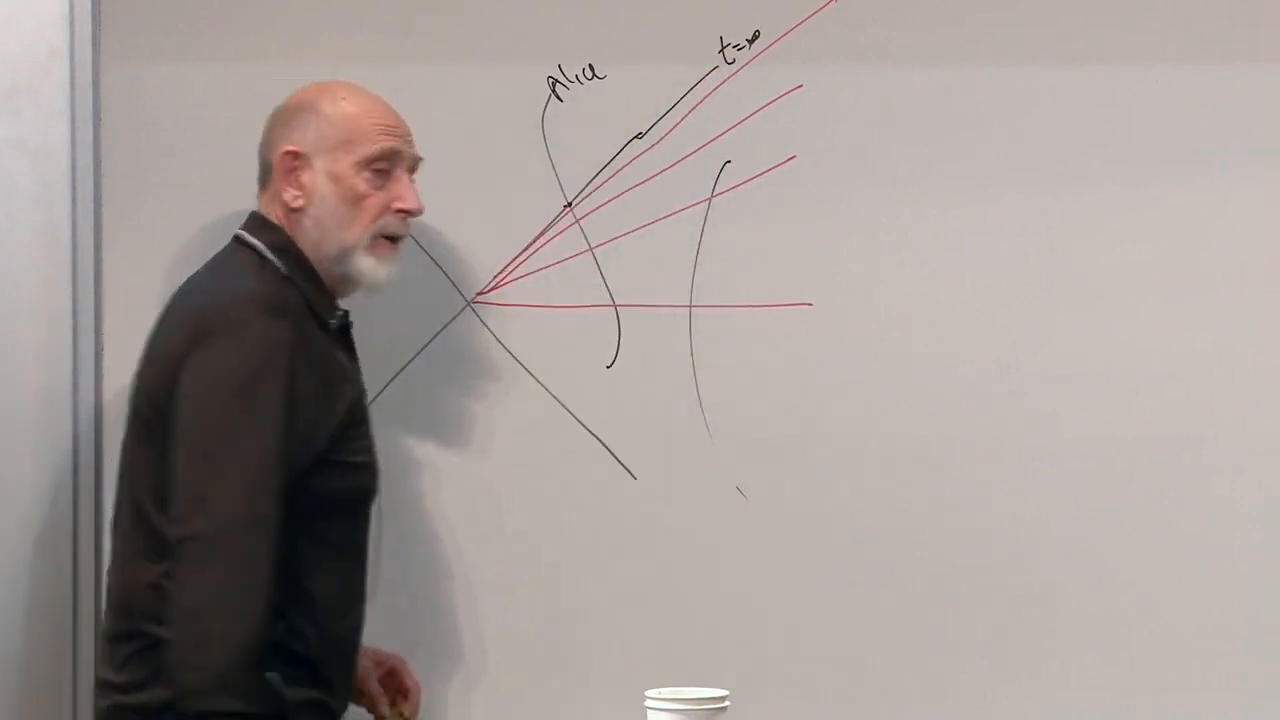
\includegraphics[width=0.84\textwidth]{lecture_07_figure_04.png}
\caption{Alices Weltlinie beim Hineinfallen und die Linien konstanter Schwarzschild-Zeit. Der Grenzstrahl ist mit \(t=\infty\) bezeichnet.}
\lectureframe{00:54:54}
\end{figure}

Alice fällt frei. Ihre Weltlinie durchquert den Horizont und erreicht die Singularität in endlicher Eigenzeit. Wenn das Schwarze Loch groß genug ist, sodass die Gezeitenkräfte dort klein sind, geschieht ihrer Uhr am Horizont nichts Besonderes.

Bob bleibt stattdessen auf einem festen Außenradius. Um dort zu verharren, muss er beschleunigen. Licht von späteren Punkten auf Alices Bahn erreicht ihn mit zunehmender Verzögerung und stärkerer Rotverschiebung. In Schwarzschild-Zeit nähert sich Alice \(t=\infty\), und Bob empfängt kein Signal, das nach ihrem Überqueren des Horizonts ausgesandt wird. Das sind Aussagen über kausale Signale und die Schwarzschild-Zeitschnitte, kein Beleg für eine materielle Oberfläche am Horizont.

\begin{classroomqa}
\audiencequestion{Wenn Bob Alice langsamer werden sieht, muss Alice dann Bob schneller werden sehen?}
\lecturerresponse{Nein. Alice empfängt weiterhin gewöhnliche Lichtsignale von Bob, solange ihre Weltlinie besteht. Auf Bobs Weltlinie gibt es ein letztes Ereignis, von dem aus ein Signal Alice erreichen kann; es ist nur deshalb das letzte, weil Alice anschließend auf die Singularität trifft. Bob geschieht nichts Abruptes. Beobachtungen blicken stets in einen vergangenen Lichtkegel, und zwischen den beiden Weltlinien besteht eine asymmetrische kausale Beziehung.
\lecturetimestamp{00:58:31--01:01:23}}
\end{classroomqa}

\begin{classroomqa}
\audiencequestion{Wenn Bob weiß, dass Alice seinen Koordinaten zufolge noch nahe am Horizont ist, kann er dann hinuntergehen, sie retten und zurückkehren?}
\lecturerresponse{Eine Rettungsweltlinie muss Alice begegnen, bevor sie den Ereignishorizont überquert. Nach diesem Ereignis kann kein zukunftsgerichteter Weg mehr zu ihr führen und anschließend wieder nach außen zurückkehren. Dass die Schwarzschild-Zeitschnitte die Überquerung bei \(t=\infty\) ansetzen, bedeutet nicht, dass Alice auf einer materiellen Oberfläche sitzt, von der man sie holen könnte; es zeigt, dass diese Zeitschnitte keinen globalen Begriff von „Jetzt“ über den Horizont hinweg liefern.
\lecturetimestamp{01:01:24--01:02:12}}
\end{classroomqa}

\section{Charlie folgt Alice}

Charlie falle Alice in geringem Abstand hinterher. Dann sind beide in Horizontnähe näherungsweise inertial. Sie können Signale austauschen, sich in beide Richtungen unterhalten oder sogar Händchen halten. Keiner von beiden findet ein Hinweisschild, das den Horizont markiert. Der Unterschied zu Bob besteht nicht darin, dass hier drei Personen mit Namen vorkommen. Er besteht im Unterschied zwischen freiem Fall und einer beschleunigten Weltlinie, die draußen bleibt.

\begin{classroomqa}
\audiencequestion{Was sieht Bob, wenn Alice zuerst fällt und Charlie ihr wie ein Basketball, der einem Reifen folgt, hinterherfällt?}
\lecturerresponse{Bob sieht beide den Horizont erreichen. Alice ist voraus und scheint daher zuerst immer stärker verlangsamt und radial gestaucht zu werden. Charlie scheint ihr immer näher zu kommen, holt sie aber in Bobs Grenzansicht von außen niemals ein. Das visuelle Aufeinanderstapeln beschreibt nicht, was einer der beiden Fallenden empfindet.
\lecturetimestamp{01:04:12--01:06:05}}
\end{classroomqa}

\begin{classroomqa}
\audiencequestion{Widerspricht die scheinbare Abflachung der Gezeitenkraft, die einen Fallenden radial dehnen müsste?}
\lecturerresponse{Das sind verschiedene Effekte. Die Abflachung gehört zu Bobs Beschreibung in Schwarzschild-Koordinaten. Die Gezeitenstreckung ist ein lokaler Krümmungseffekt, den Alice und Charlie spüren können. Bei der Diskussion der Beobachter wird ein hinreichend großes Schwarzes Loch oder hinreichend kleine Beobachter vorausgesetzt, sodass der Gezeiteneffekt am Horizont vernachlässigbar ist. Bei einem Schwarzen Loch von ungefähr einer Sonnenmasse wären die Gezeitenkräfte am Horizont stattdessen enorm, während sie bei einem supermassereichen Loch schwach sein können.
\lecturetimestamp{01:06:07--01:08:18}}
\end{classroomqa}

\begin{classroomqa}
\audiencequestion{Sieht Charlie Alice den Horizont überqueren, solange er selbst noch draußen ist?}
\lecturerresponse{Zeichnen Sie den lichtartigen Strahl ein. Das beim Überqueren durch Alice ausgesandte Licht verläuft entlang des Horizonts und erreicht Charlie, wenn er selbst den Horizont überquert. An diesem Ereignis kann er berechnen, dass er ihr Überqueren gesehen hat, obwohl keiner der beiden Beobachter vor Ort eine Markierung wahrnimmt. Danach kann er sie im Inneren sehen. Beschleunigt er vor dem Überqueren weg und schafft es, draußen zu bleiben, sieht er das Überqueren nicht.
\lecturetimestamp{01:08:19--01:11:11}}
\end{classroomqa}

\begin{classroomqa}
\audiencequestion{Wenn Alice bereits im Inneren und Charlie noch draußen ist, wie lassen sich dann ihre späteren Radien und Überquerungszeiten vergleichen?}
\lecturerresponse{Aus einer Formulierung wie „zur selben Zeit“ lässt sich keine beobachterunabhängige Gleichzeitigkeit ablesen. Alice sieht Charlie auf ihrem vergangenen Lichtkegel und kann sein späteres Überqueren erst sehen, wenn sie sich weiter im Inneren befindet. Die konkrete Weltlinien und lichtartigen Strahlen beantworten die Frage. Eine weitergehende Verallgemeinerung auf viele weit voneinander entfernte Fallende muss anhand ihres tatsächlichen kausalen Diagramms überprüft werden; man darf nicht einfach eine universelle Überquerungszeit voraussetzen.
\lecturetimestamp{01:11:14--01:12:31}}
\end{classroomqa}

In den regulären Koordinaten nahe am Horizont verläuft eine Freifallbahn nahezu geradlinig. In der vollständigen Schwarzschild-Geometrie ist sie nicht exakt gerade, doch nahe einem großen, schwach gekrümmten Horizont ist diese Näherung gut.

\begin{classroomqa}
\audiencequestion{Kann die Stringtheorie klären, was im Inneren eines Schwarzen Lochs im Bereich der Quantengravitation geschieht?}
\lecturerresponse{Genau dort wird das Thema heikel. In der Nähe der Singularität ist eine Quantentheorie der Gravitation erforderlich, und die Stringtheorie ist ein möglicher Rahmen dafür. Die einschlägigen Fragen waren jedoch offen und schwierig; sie ließen sich nicht durch eine einfache Anwendung des klassischen Diagramms lösen.
\lecturetimestamp{01:13:04--01:13:38}}
\end{classroomqa}

\begin{classroomqa}
\audiencequestion{Was geschieht mit Alices eigener Uhr und Geschwindigkeit, wenn sie den Horizont überquert?}
\lecturerresponse{Ihre Uhr tickt weiterhin mit ihrer gewöhnlichen lokalen Rate und zeigt eine endliche Eigenzeit an. In ihrem momentanen Ruhesystem ist sie in Ruhe; relativ zu einem lokalen frei fallenden Bezugssystem hat sie eine gewöhnliche endliche Geschwindigkeit. Nahe einem großen Horizont ist die Geometrie nahezu flach, sodass die Markierungen gleicher Eigenzeit entlang ihrer Weltlinie regulär bleiben, bis die Krümmung nahe der Singularität stark wird.
\lecturetimestamp{01:13:39--01:14:44}}
\end{classroomqa}

\begin{classroomqa}
\audiencequestion{Was, wenn Bob sich nach außen beschleunigt, aber nicht stark genug, um das Hindurchfallen zu verhindern?}
\lecturerresponse{Dann biegt sich seine Weltlinie nach außen, überquert aber dennoch den Horizont. Überquert er ihn sehr spät, kann er Alice kurz nach ihrem Überqueren sehen; bis zur Singularität bleibt ihm dann jedoch nur eine kurze Eigenzeit. Die Steigungen der Weltlinien in der Skizze sind keine geeichten Maßstäbe oder Uhren; erhalten bleibt die kausale Reihenfolge, nicht ihre gezeichnete euklidische Länge.
\lecturetimestamp{01:14:47--01:16:31}}
\end{classroomqa}

Alle diese Schlussfolgerungen setzen voraus, dass kein Signal das Licht überholt. In der Vorlesung werden kurz die damals jüngsten Presseberichte über scheinbar überlichtschnelle Neutrinos in Italien scherzhaft erwähnt – ein Verweis auf einen Fehler bei der experimentellen Zeitmessung, nicht auf eine Ausnahme von der Relativitätstheorie. Die kausale Konstruktion selbst bleibt durch die lichtartigen Geraden begrenzt.

\begin{classroomqa}
\audiencequestion{Können mitgeführte, synchronisierte Uhren von Alice und Bob die Frage entscheiden, wenn Alice zum Horizont hinabtaucht und zurückkehrt?}
\lecturerresponse{Wenn ihre Weltlinien zusammentreffen, können sie ihre Uhren vergleichen. Sobald sie sich jedoch trennen, gibt es keine eindeutige Synchronisation über räumliche Entfernung hinweg, insbesondere wenn einer seinen Bewegungszustand ändert. Zeichnen Sie beide Weltlinien und die ausgetauschten lichtartigen Strahlen ein. Für jedes genau festgelegte Experiment liefert dieses Diagramm die operative Antwort.
\lecturetimestamp{01:17:34--01:18:25}}
\end{classroomqa}

\begin{figure}[htbp]
\centering
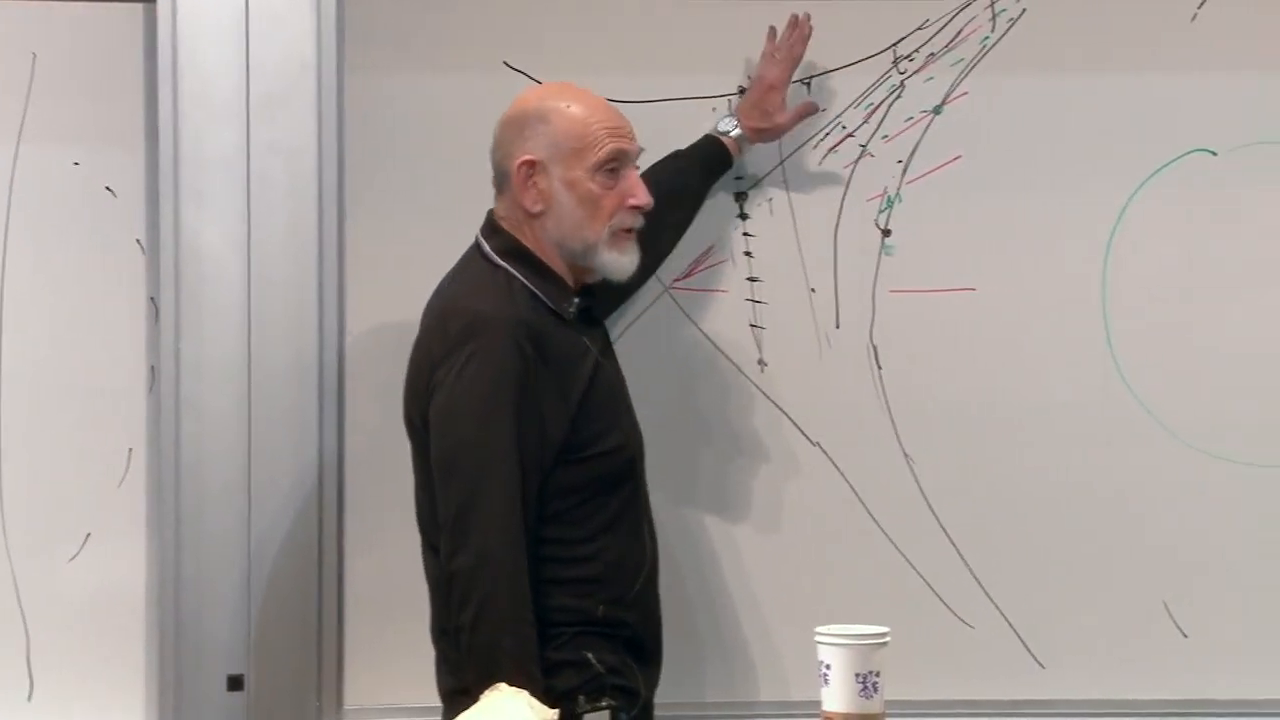
\includegraphics[width=0.86\textwidth]{lecture_07_figure_05.png}
\caption{Das vervollständigte kausale Diagramm, mit dem die Fragen zu Alice, Bob und Charlie beantwortet werden. Jede Beobachtung wird lokalisiert, indem man vom beobachteten Ereignis einen lichtartigen Strahl bis zur Weltlinie des Beobachters zurückverfolgt.}
\lectureframe{01:18:12}
\end{figure}

\begin{figure}[htbp]
\centering
\resizebox{0.96\linewidth}{!}{%
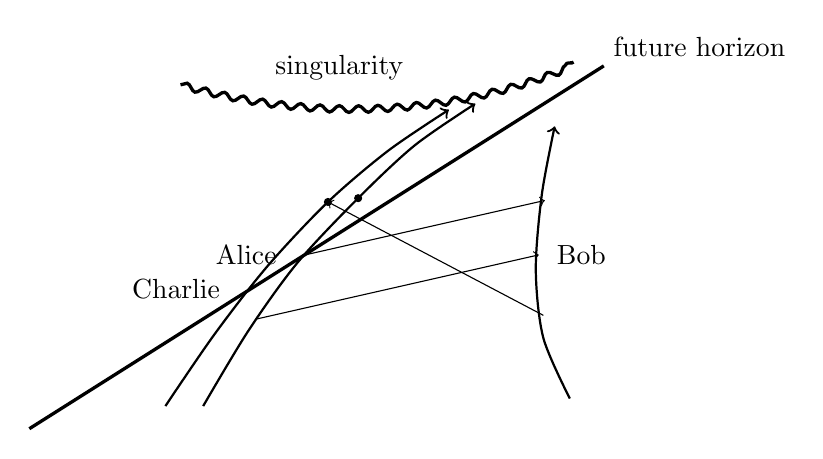
\begin{tikzpicture}[scale=0.96]
\draw[very thick] (-3.8,-0.3) -- (3.8,4.5);
\node[above right] at (3.8,4.5) {future horizon};
\draw[very thick,decorate,decoration={snake,amplitude=1.2pt,segment length=7pt}]
  (-1.8,4.25) .. controls (0.1,3.72) and (2.0,3.92) .. (3.4,4.55);
\node at (0.3,4.48) {singularity};
\draw[thick,->]
  plot[smooth] coordinates {(-1.5,0.0) (-0.9,1.0) (-0.25,1.9)
  (0.55,2.75) (1.3,3.45) (2.1,4.0)};
\node[left] at (-0.4,2.0) {Alice};
\draw[thick,->]
  plot[smooth] coordinates {(-2.0,0.0) (-1.35,0.95) (-0.65,1.85)
  (0.15,2.7) (0.95,3.38) (1.75,3.92)};
\node[left] at (-1.15,1.55) {Charlie};
\draw[thick,->]
  plot[smooth] coordinates {(3.35,0.1) (3.0,0.9) (2.9,1.8)
  (2.98,2.8) (3.15,3.7)};
\node[right] at (3.05,2.0) {Bob};
\draw[thin,->] (-0.8,1.15) -- (2.94,2.0);
\draw[thin,->] (-0.15,2.0) -- (3.02,2.72);
\draw[thin,->] (3.0,1.2) -- (0.15,2.7);
\draw[fill] (0.55,2.75) circle (1.3pt);
\draw[fill] (0.15,2.7) circle (1.3pt);
\end{tikzpicture}
}
\caption{Ein schematisches Beobachterdiagramm. Bobs Beobachtungen von außen und die gegenseitigen Beobachtungen von Alice und Charlie ergeben sich aus unterschiedlichen lichtartigen Strahlen; sie lassen sich nicht auf wechselseitige Schlagworte über Uhren reduzieren.}
\label{fig:l7-observers-clean}
\end{figure}

\begin{classroomqa}
\audiencequestion{Sieht Bob Alice unendlich lange, und bedeutet das, dass sie in seiner Wirklichkeit nie stirbt?}
\lecturerresponse{Bob empfängt ihre Signale während eines unbegrenzten Zeitintervalls seiner eigenen Zeit, doch er sieht, wie ihre Uhr immer langsamer bis zum Stillstand zu gehen scheint, und empfängt nur die endliche Folge der Herzschläge, die vor ihrem Überqueren ausgesandt wurden. Das Wort „Wirklichkeit“ verschleiert den Unterschied zwischen einem lokalen Ereignis und dem asymptotischen Beobachtungsprotokoll eines Beobachters. Alice erlebt am Horizont keinen Uhrenstillstand; Bobs Aufzeichnungen treffen mit immer größerer Verzögerung und stärkerer Rotverschiebung ein.
\lecturetimestamp{01:18:32--01:20:59}}
\end{classroomqa}

\begin{classroomqa}
\audiencequestion{Sieht Alice plötzlich all die alte Materie, die am Horizont eingefroren zu sein schien, sobald sie ihn überquert?}
\lecturerresponse{Nichts wird plötzlich frei sichtbar. Während sie fällt, ändern sich die vergangenen Lichtkegel, über die sie frühere Materie sieht, stetig. Sie kann folgern, dass das Licht, das sie jetzt erreicht, früher ausgesandt wurde und dass die Materie vor ihr den Horizont überquert hat. Charlies Blick auf Alice lehrt dasselbe: Beim Überqueren entsteht für keinen der beiden ein lokaler Sprung, und es wird auch kein verborgener Haufen aus Stühlen und Dinosauriern sichtbar.
\lecturetimestamp{01:21:02--01:23:48}}
\end{classroomqa}

\begin{classroomqa}
\audiencequestion{Gibt es realistische Simulationen dessen, was ein Fallender sehen würde?}
\lecturerresponse{In der Vorlesung wird auf Andrew Hamiltons Visualisierungen Schwarzer Löcher verwiesen. Sie können die starke Aberration und die Frequenzverschiebungen einfallenden Lichts veranschaulichen, auch wenn die Darstellung eher verwirrend als erhellend sein kann. „Nichts Besonderes am Horizont“ bezieht sich auf die lokale Geometrie, nicht darauf, dass der Himmel gewöhnlich aussieht.
\lecturetimestamp{01:24:11--01:25:29}}
\end{classroomqa}

\section{Vom ewigen zum wachsenden Schwarzen Loch}

Die untere Spitze des maximal fortgesetzten Diagramms des ewigen Schwarzen Lochs hat für ein durch Sternkollaps entstandenes Schwarzes Loch kaum unmittelbare Bedeutung. In der einfachen Kollapsgeometrie tritt nur der Teil mit dem Außenbereich, dem zukünftigen Horizont und dem zukünftigen Inneren auf. Dieser Unterschied wird entscheidend, sobald Materie die Masse des Lochs verändern darf.

\begin{classroomqa}
\audiencequestion{Welches physikalische Ereignis stellt die untere Spitze des idealisierten Diagramms dar?}
\lecturerresponse{Für die ewige mathematische Lösung ist sie Teil der maximalen Fortsetzung. Ein aus kollabierender Materie entstandenes Schwarzes Loch enthält nicht den gesamten unteren Bereich. Sein Horizont hat eine Entstehungsgeschichte, für die ein anderes globales Diagramm erforderlich ist; sie wird in der nächsten Vorlesung behandelt.
\lecturetimestamp{01:25:59--01:26:52}}
\end{classroomqa}

Wenn ein kleiner Testkörper hineinfällt, kann man seine Rückwirkung vernachlässigen, und das feste Schwarzschild-Diagramm genügt. Fällt eine beträchtliche Masse hinein, nehmen die Masse des Schwarzen Lochs und sein Schwarzschild-Radius zu:
\begin{equation}
r_{\mathrm S}=2GM,
\qquad
\Delta r_{\mathrm S}=2G\,\Delta M.
\label{eq:l7-growing-radius}
\end{equation}
Der Horizont verformt sich in Richtung des einfallenden Objekts, die Horizonte vereinigen sich, und der verformte gemeinsame Horizont stellt rasch einen stationären Zustand her. In der nichtrotierenden Idealisierung der Vorlesung ist das Ergebnis eine etwas größere Kugel. Bei einer tatsächlichen Verschmelzung wird außerdem Energie in Form von Gravitationswellen abgestrahlt, und im Allgemeinen bleibt ein rotierendes Loch zurück.

\begin{classroomqa}
\audiencequestion{Wenn der Horizont beim Einfallen von Masse wächst, bewegt er sich dann nach außen, um Materie zu erreichen, die nahe dem alten Horizont eingefroren zu sein schien?}
\lecturerresponse{Für einen hinreichend massereichen einfallenden Körper gilt die Testteilchen-Näherung nicht mehr. Der Horizont verformt sich, vereinigt sich mit dem gefangenen Bereich des einfallenden Körpers und geht in einen größeren stationären Horizont über. Die genaue Lage des Ereignishorizonts ist global bestimmt und kann sich in einen Bereich erstrecken, bevor die einfallende Materie dort eintrifft. Die Vorlesung stellt die vollständige Konstruktion bewusst zurück und behandelt sie in der nächsten Sitzung.
\lecturetimestamp{01:26:55--01:29:05}}
\end{classroomqa}

\begin{classroomqa}
\audiencequestion{Warum können Astronomen Lichtblitze sehen, wenn Materie angeblich unendlich viel Schwarzschild-Zeit braucht, um den Horizont zu erreichen?}
\lecturerresponse{Die helle Strahlung stammt nicht vom Horizont selbst. Gas in einer Akkretionsströmung oder -scheibe stößt zusammen und erhitzt sich außerhalb des Horizonts, auch in der Nähe starker Photonbahnen. Dieses Plasma außerhalb des Horizonts kann Licht aussenden, das uns erreicht. Die leere Schwarzschild-Geometrie isoliert das Kausalitätsproblem, ist aber kein vollständiges Modell einer astrophysikalischen Umgebung.
\lecturetimestamp{01:29:07--01:30:22}}
\end{classroomqa}

Die charakteristische Relaxationszeit wird durch die Lichtlaufzeit festgelegt:
\begin{equation}
t_{\mathrm{cross}}\sim\frac{r_{\mathrm S}}{c},
\qquad
t_{\mathrm{relax}}\sim
\text{a few to a few tens of }t_{\mathrm{cross}}.
\label{eq:l7-relaxation-scale}
\end{equation}
Die Vorlesung schätzt \(10^{-5}\,\mathrm{s}\) als Durchquerungszeit eines Lochs von der Größenordnung eines Kilometers und ungefähr \(10^{-3}\,\mathrm{s}\), bis eine kleine Verschmelzung nahezu stationär ist. Bei einem Loch mit einer Milliarde Sonnenmassen liegt die entsprechende Zeit im Bereich von Minuten bis Stunden. Das sind Skalierungsabschätzungen, keine präzisen Verschmelzungsrechnungen. Entscheidend ist die geometrische Abfolge: Hantelform, Erdnussform, nahezu kugelförmig, stationär.

\begin{classroomqa}
\audiencequestion{Wie schnell beruhigt sich ein verformter oder neu entstandener Horizont?}
\lecturerresponse{Auf einer Zeitskala, die nicht viel länger ist, als das Licht braucht, um das Loch zu durchqueren. Da alle Längen und Zeiten mit \(r_{\mathrm S}\) skalieren, beruhigen sich kleine Löcher in Sekundenbruchteilen, supermassereiche Löcher hingegen erst nach deutlich längerer Zeit. Die Aussage des No-Hair-Theorems beschreibt den stationären Endzustand; die vorübergehende Verformung trägt Energie in Form von Gravitationsstrahlung davon.
\lecturetimestamp{01:30:26--01:33:18}}
\end{classroomqa}

\begin{classroomqa}
\audiencequestion{Was sieht Bob, wenn frühere Materie zwischen altem und neuem Horizont liegt, während ein weiterer schwerer Körper hineinfällt?}
\lecturerresponse{Diese Frage lässt sich nicht konsistent beantworten, indem man zwei statische Schwarzschild-Diagramme zusammenstückelt. Man muss die zeitabhängige Kollapsgeometrie lösen oder konstruieren und ihren globalen Horizont bestimmen. Die Vorlesung hält die Frage offen und verschiebt die Antwort ausdrücklich auf die nächste Woche, wenn die Horizontentstehung behandelt wird.
\lecturetimestamp{01:33:20--01:35:41}}
\end{classroomqa}

\section{Was ändert sich bei einer Änderung des Maßstabs?}

Das dimensionslose Diagramm ändert sich nicht, wenn sich \(r_{\mathrm S}\) ändert. Wohl aber ändert sich die physikalische Bedeutung eines eingezeichneten Intervalls:
\begin{equation}
d\tau_{\mathrm{physical}}^2
=
r_{\mathrm S}^2\,d\hat{\tau}^2,
\qquad
\ell_{\mathrm{physical}}
=
r_{\mathrm S}\,\hat{\ell}.
\label{eq:l7-scale-restoration}
\end{equation}
Ein dimensionsloser Abstand, der bei einem Loch von der Größenordnung eines Kilometers einem halben Kilometer entspricht, steht bei einem um den Faktor einer Milliarde größeren Loch für ungefähr eine halbe Milliarde Kilometer. Damit kehrt die Analogie mit gleich gezeichneten Kugeln zurück: Die Form bleibt gleich, während die Zahl der Meterstäbe, die einer Linie entsprechen, mit dem Radius skaliert.

\begin{classroomqa}
\audiencequestion{Wie ändert sich das Kausaldiagramm, wenn sich der Schwarzschild-Radius ändert?}
\lecturerresponse{Es ändert sich nicht, nachdem der Radius herausfaktorisiert wurde. Jede physikalische Länge und Zeit, die dem Diagramm zugeordnet wird, wird mit \(r_{\mathrm S}\) multipliziert; die Krümmung an entsprechenden dimensionslosen Punkten dagegen mit \(r_{\mathrm S}^{-2}\).
\lecturetimestamp{01:35:41--01:38:10}}
\end{classroomqa}

\begin{classroomqa}
\audiencequestion{Ändert sich die kausale Schlussfolgerung, wenn Bob eine Umlaufbahn beschreibt, statt an einer festen Winkelposition zu schweben?}
\lecturerresponse{Die Einzelheiten der Rotverschiebung und der Ankunftsrichtungen werden komplizierter, doch die kausale Trennung durch den Horizont ändert sich nicht. Keine zeitartige Bahn außerhalb des Horizonts empfängt ein Signal, das von innerhalb des Horizonts ausgesandt wurde.
\lecturetimestamp{01:38:12--01:38:26}}
\end{classroomqa}

\begin{classroomqa}
\audiencequestion{Da die Gravitation innerhalb einer Kugelschale verschwindet: Verschwindet sie auch innerhalb des Horizonts, weil die Masse des Schwarzen Lochs über diese Oberfläche verteilt ist?}
\lecturerresponse{Nein. Der Ereignishorizont ist keine materielle Schale, die die Masse trägt. Der Newtonsche Schalentheorem ist daher auf ihn nicht anwendbar. Die Vorlesung vergleicht die statische Außenlösung mit einer Punktquelle an der Krümmungssingularität. Während der Entstehung einfallende Materie erfordert jedoch die zeitabhängige Geometrie, die erst in der nächsten Vorlesung behandelt wird.
\lecturetimestamp{01:38:28--01:40:41}}
\end{classroomqa}

\section{Rotation und radiale Geometrie}

Der Drehimpuls bleibt beim Kollaps erhalten. Ein rotierendes Schwarzes Loch besitzt eine andere Außengeometrie als die Schwarzschild-Lösung: Seine stationäre Lösung ist die Kerr-Lösung, die Rotation verzerrt die Geometrie des Horizonts, und die Mitführung der Bezugssysteme dreht die Trägheitsrichtungen um das Loch. Im Prinzip lässt sich der Drehimpuls anhand dieser gravitativen Effekte außerhalb des Lochs messen. Materie verliert ihren Drehimpuls nicht einfach dadurch, dass sie einen Horizont überschreitet.

\begin{classroomqa}
\audiencequestion{Kann ein Schwarzes Loch einen messbaren Drehimpuls besitzen, und verändert die Rotation die Gravitation außerhalb des Lochs?}
\lecturerresponse{Ja. Der Drehimpuls bleibt als Erhaltungsparameter bestehen, verformt die stationäre Geometrie und bewirkt eine Mitführung der Bezugssysteme. Der Horizont ist dann nicht mehr der einfache kugelförmige Schwarzschild-Horizont. Die Vorlesung vergleicht die Verformung qualitativ mit der abgeplatteten Form der Erde und weist zugleich darauf hin, dass die vollständige rotierende Lösung wesentlich komplizierter ist.
\lecturetimestamp{01:40:45--01:42:36}}
\end{classroomqa}

\begin{classroomqa}
\audiencequestion{Bedeutet die Beziehung zwischen \(r\) und der Eigenlänge \(\rho\)}, dass die Gravitation den Raum kontrahiert?\lecturerresponse{Die radiale Eigenlänge \(\rho\) erfüllt
\begin{equation*}
\frac{d\rho}{dr}=\sqrt{\frac{r}{r-1}}>1
\end{equation*}außerhalb des Einheitshorizonts die folgende Beziehung. Ein gegebenes Koordinatenintervall \(dr\) entspricht daher in Horizontnähe einem größeren radialen Eigenlängenintervall. Ob man von einem kontrahierten oder gedehnten Raum spricht, hängt davon ab, welche Koordinatenintervalle man vergleicht. Die invariante Aussage ist die Beziehung zwischen den Eigenlängen selbst.
\lecturetimestamp{01:42:36--01:43:20}}
\end{classroomqa}

\section{Abschließende Fragen}

\begin{classroomqa}
\audiencequestion{Aus Bobs Sicht nähert sich Alices Uhr dem Stillstand. Endet aus Alices Sicht Bobs Raum oder Zeit?}
\lecturerresponse{Nein. Alice sieht gewöhnliche Signale von aufeinanderfolgenden Ereignissen auf Bobs Weltlinie, bis ihre eigene Weltlinie endet. Sie sieht keine späteren Ereignisse von Bob, weil es auf ihrer Weltlinie keinen späteren Punkt gibt, nicht weil Bob oder sein Raum verschwindet. In diesen regulären kausalen Koordinaten verlaufen radiale Lichtstrahlen geradlinig; dass sie in einem anderen Koordinatensystem als gekrümmte Bahnen erscheinen, ändert nichts daran, welche Ereignisse sie verbinden.
\lecturetimestamp{01:43:21--01:45:20}}
\end{classroomqa}

Die allgemeine Relativitätstheorie stellt zwei einander ergänzende Aufgaben. Ist eine Metrik gegeben, lassen sich Geodäten und lichtartige Strahlen verfolgen, um zu bestimmen, was Beobachter messen. Ist eine Materieverteilung gegeben, müssen die Einsteinschen Feldgleichungen gelöst werden, um die Metrik zu finden. Mit der ersten Aufgabe hat sich diese Vorlesung befasst. Die zweite ist gewöhnlich schwieriger, auch wenn symmetrischer Kollaps handhabbare Beispiele liefert.

\begin{classroomqa}
\audiencequestion{Was geschieht mit dem Horizont und der Singularität eines verdampfenden Schwarzen Lochs?}
\lecturerresponse{Die Vorlesung zeigt eine schematische Darstellung, in der der Horizont schrumpft und auf den Endpunkt des Singularitätsbereichs trifft. Die Verdampfung ist ein semiklassischer Quantenprozess, und was am Ende auf der Planck-Skala geschieht, lässt sich aus dem klassischen Schwarzschild-Diagramm nicht bestimmen. Die Skizze des schrumpfenden Horizonts ist daher als qualitativer Ausblick zu verstehen, nicht als vollständige Quantengeometrie.
\lecturetimestamp{01:46:04--01:46:32}}
\end{classroomqa}

Fast jedes Schwarze Loch in der Astrophysik dürfte rotieren. Sterne besitzen bereits Drehimpuls, und beim Kollaps nimmt ihre Winkelgeschwindigkeit in der bekannten Weise zu, wie bei einer Eiskunstläuferin, die die Arme an den Körper zieht. Die Singularitätsstruktur eines Kerr-Schwarzen Lochs ist nicht die hier dargestellte Schwarzschild-\(r=0\)-Fläche und sollte nicht so beschrieben werden, als rotiere Materie buchstäblich mit unendlicher Bahngeschwindigkeit.

\begin{classroomqa}
\audiencequestion{Sind nichtrotierende Schwarze Löcher makroskopischer Größe häufig, und wie viele Schwarze Löcher gibt es?}
\lecturerresponse{Ein Drehimpuls von exakt null wäre eine außergewöhnliche Idealisierung. Die Vorlesung nennt lediglich eine grobe Schätzung für den Unterricht zur Größenordnung der kosmischen Population: Sie liegt zwischen der Zahl der Galaxien und der Zahl der Sterne und vielleicht bei ungefähr \(10^{15}\). Das ist eine Schätzung aus der Zeit der Vorlesung, keine durch Zählung ermittelte Bestandsaufnahme. Entscheidend ist, dass beim Kollaps im Allgemeinen ein gewisser Drehimpuls erhalten bleibt und zunimmt.
\lecturetimestamp{01:46:32--01:48:42}}
\end{classroomqa}

\begin{classroomqa}
\audiencequestion{Entstehen Schwarze Löcher aus bereits vorhandener Materie oder durch einen Quantenprozess?}
\lecturerresponse{Gewöhnliche astrophysikalische Schwarze Löcher entstehen, wenn bereits vorhandene Sternmaterie kollabiert. Kernfusion und der nach außen gerichtete Energiefluss tragen dazu bei, einen Stern zu stützen. Ist der Brennstoff erschöpft, zieht sich der Überrest zusammen. Je nach seiner Masse und der verfügbaren Druckstützung kann er zu einem Weißen Zwerg oder einem Neutronenstern werden oder, falls keine Stützung den Kollaps aufhalten kann, seinen eigenen Schwarzschild-Radius unterschreiten und ein Schwarzes Loch bilden.
\lecturetimestamp{01:48:43--01:50:23}}
\end{classroomqa}

\begin{classroomqa}
\audiencequestion{Können mikroskopische Schwarze Löcher entstehen, und wovon hängen ihre Lebensdauer und ihre Mindestgröße ab?}
\lecturerresponse{Dieser Teil ist spekulativ. Die Hawking-Verdampfung verläuft bei geringerer Masse schneller; die Lebensdauer skaliert näherungsweise wie \(M^3\). Die Vorlesung vergleicht ein Loch mit einem Berg an Masse, dessen Lebensdauer kosmologische Größenordnung haben könnte; diese Zahlenanalogie ist nur grob. Starke Dichteschwankungen im frühen Universum oder hinreichend energiereiche Kollisionen sind denkbare Entstehungsmechanismen. Ein Schwarzes Loch nahe der Planck-Masse, ungefähr \(10^{-5}\,\mathrm{g}\), kennzeichnet die Skala, ab der eine klassische geometrische Beschreibung nicht mehr verlässlich ist. Bei einer einfachen Extrapolation würde man für diese Energie einen unplausibel großen gewöhnlichen Beschleuniger benötigen, auch wenn eine solche Entstehung prinzipiell möglich ist.
\lecturetimestamp{01:50:23--01:53:31}}
\end{classroomqa}

\begin{classroomqa}
\audiencequestion{Wird der Kurs noch Kosmologie, dunkle Materie, dunkle Energie, Entropie und Gravitationswellen behandeln?}
\lecturerresponse{Kosmologische Anwendungen und vielleicht auch Gravitationswellen könnten spätere Themen sein. Die Entropie Schwarzer Löcher wird auf die Zeit nach diesem Vierteljahr verschoben. Zum Schluss räumt die Vorlesung ein, dass an diesem Abend nur etwa ein Viertel des geplanten Stoffes behandelt wurde: Die Fragen sorgfältig zu klären ist wichtiger, als die Gliederung im Eiltempo durchzugehen.
\lecturetimestamp{01:53:33--01:54:38}}
\end{classroomqa}

Die handlungsleitende Regel bewährt sich bei jeder Frage im Hörsaal. Man legt die Weltlinien fest, zeichnet die lichtartigen Strahlen ein und bestimmt die Ereignisse, die sie verbinden. Am Horizont versagt die lokale Physik nicht; er ist die Grenze, jenseits deren jedes zukunftsgerichtete Signal innerhalb des Horizonts bleibt. In der nächsten Vorlesung wird der ewige Hintergrund durch eine kollabierende Quelle ersetzt und gezeigt, wie diese Grenze entsteht.